../cictikz/src/cictikz/data/tex/cictikz_preamble.tex

% Where the return current actually flows, drawn on a real board: a
% copper trace over a ground plane, in oblique view. At DC the return
% spreads across the plane; at high frequency it crowds into a band
% directly under the trace - smallest loop, smallest inductance. The
% shading is the current density in the plane.

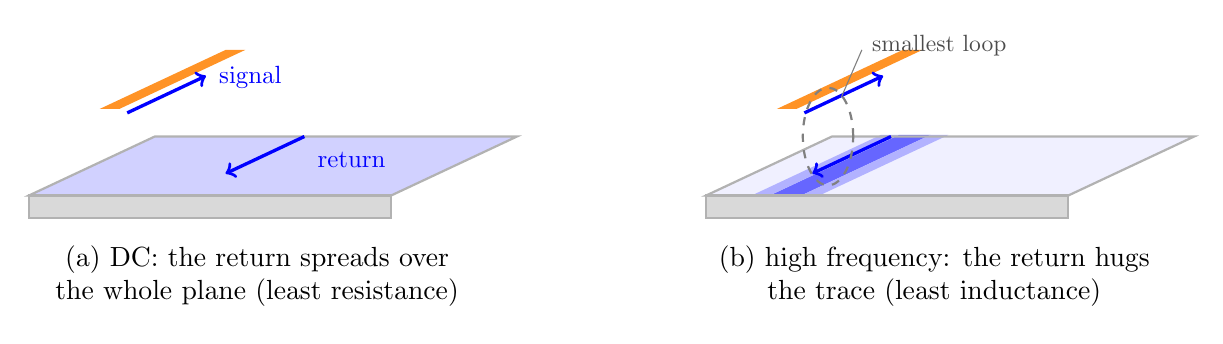
\begin{tikzpicture}[thick]

  \def\dx{1.6}
  \def\dy{0.75}

  % ---------------- (a) DC ----------------
  % plane slab, uniformly tinted: the return spreads
  \fill[blue!18] (0,0) -- (4.6,0) -- (4.6+\dx,\dy) -- (\dx,\dy) -- cycle;
  \draw[gray!60] (0,0) -- (4.6,0) -- (4.6+\dx,\dy) -- (\dx,\dy) -- cycle;
  \fill[gray!30] (0,-0.28) rectangle (4.6,0);
  \draw[gray!60] (0,-0.28) rectangle (4.6,0);
  % the trace floating above, running the same direction
  \fill[orange!85] (0.9,1.1) -- (1.15,1.1) -- (1.15+\dx,1.1+\dy) -- (0.9+\dx,1.1+\dy) -- cycle;
  \draw[blue, very thick, ->] (1.25,1.05) -- (2.25,1.52);
  \node[blue, anchor=west, scale=0.9] at (2.3,1.5) {signal};
  \draw[blue, very thick, <-] (2.5,0.28) -- (3.5,0.75);
  \node[blue, anchor=west, scale=0.9] at (3.55,0.45) {return};
  \node[anchor=north, align=center] at (2.9,-0.5)
    {(a) DC: the return spreads over\\the whole plane (least resistance)};

  % ---------------- (b) high frequency ----------------
  \begin{scope}[shift={(8.6,0)}]
    \fill[blue!6] (0,0) -- (4.6,0) -- (4.6+\dx,\dy) -- (\dx,\dy) -- cycle;
    % the density crowds under the trace: a shaded band along it
    \fill[blue!60] (0.85,0.02) -- (1.25,0.02) -- (1.25+\dx,0.02+\dy) -- (0.85+\dx,0.02+\dy) -- cycle;
    \fill[blue!30] (0.62,0.02) -- (0.85,0.02) -- (0.85+\dx,0.02+\dy) -- (0.62+\dx,0.02+\dy) -- cycle;
    \fill[blue!30] (1.25,0.02) -- (1.48,0.02) -- (1.48+\dx,0.02+\dy) -- (1.25+\dx,0.02+\dy) -- cycle;
    \draw[gray!60] (0,0) -- (4.6,0) -- (4.6+\dx,\dy) -- (\dx,\dy) -- cycle;
    \fill[gray!30] (0,-0.28) rectangle (4.6,0);
    \draw[gray!60] (0,-0.28) rectangle (4.6,0);
    \fill[orange!85] (0.9,1.1) -- (1.15,1.1) -- (1.15+\dx,1.1+\dy) -- (0.9+\dx,1.1+\dy) -- cycle;
    \draw[blue, very thick, ->] (1.25,1.05) -- (2.25,1.52);
    \draw[blue, very thick, <-] (1.35,0.28) -- (2.35,0.75);
    % the loop being minimized
    \draw[gray, dashed, thick] (1.55,0.75) ellipse (0.32 and 0.62);
    \node[gray!60!black, anchor=west, scale=0.85] at (2.0,1.9) {smallest loop};
    \draw[gray, thin] (1.98,1.85) -- (1.72,1.25);
    \node[anchor=north, align=center] at (2.9,-0.5)
      {(b) high frequency: the return hugs\\the trace (least inductance)};
  \end{scope}

\end{tikzpicture}
\end{document}
